% GoldenHour — Technical Documentation
% Bharat Academix CodeQuest 2026 — MVP Submission
% Compile on Overleaf with pdfLaTeX. No external assets required.

\documentclass[11pt]{article}

% ---------- Packages -------------------------------------------------------
\usepackage[a4paper,margin=2.3cm]{geometry}
\usepackage[T1]{fontenc}
\usepackage{lmodern}
\usepackage{microtype}
\usepackage{xcolor}
\usepackage{graphicx}
\usepackage{booktabs}
\usepackage{tabularx}
\usepackage{array}
\usepackage{amsmath}
\usepackage{enumitem}
\usepackage{titlesec}
\usepackage{fancyhdr}
\usepackage{listings}
\usepackage{tikz}
\usetikzlibrary{shapes.geometric, arrows.meta, positioning, calc, fit, backgrounds}
\usepackage[hidelinks]{hyperref}

% ---------- Brand palette --------------------------------------------------
\definecolor{ghAmber}{HTML}{F59E0B}
\definecolor{ghCrimson}{HTML}{DC2626}
\definecolor{ghEmerald}{HTML}{10B981}
\definecolor{ghInk}{HTML}{1A1A1A}
\definecolor{ghSlate}{HTML}{475569}
\definecolor{ghSlateLight}{HTML}{E2E8F0}
\definecolor{ghBgSoft}{HTML}{FBF7F0}
\definecolor{ghCodeBg}{HTML}{F6F8FA}

\hypersetup{
  colorlinks=true,
  linkcolor=ghCrimson,
  urlcolor=ghCrimson,
  citecolor=ghCrimson,
  pdftitle={GoldenHour --- Technical Documentation},
  pdfauthor={Team GoldenHour}
}

% ---------- Section styling ------------------------------------------------
\titleformat{\section}
  {\color{ghInk}\Large\bfseries\sffamily}
  {\color{ghAmber}\thesection}{0.6em}{}
  [\vspace{2pt}{\color{ghAmber}\titlerule[1.2pt]}]
\titleformat{\subsection}
  {\color{ghInk}\large\bfseries\sffamily}
  {\color{ghCrimson}\thesubsection}{0.6em}{}
\titlespacing*{\section}{0pt}{14pt}{8pt}
\titlespacing*{\subsection}{0pt}{10pt}{4pt}

% ---------- Header / footer ------------------------------------------------
\pagestyle{fancy}
\fancyhf{}
\renewcommand{\headrulewidth}{0.4pt}
\renewcommand{\footrulewidth}{0.4pt}
\fancyhead[L]{\small\sffamily\color{ghSlate}GoldenHour}
\fancyhead[R]{\small\sffamily\color{ghSlate}Technical Documentation}
\fancyfoot[L]{\small\sffamily\color{ghSlate}Bharat Academix CodeQuest 2026}
\fancyfoot[R]{\small\sffamily\color{ghSlate}\thepage}

% ---------- Code listing style ---------------------------------------------
\lstdefinestyle{gh}{
  backgroundcolor=\color{ghCodeBg},
  basicstyle=\ttfamily\footnotesize\color{ghInk},
  keywordstyle=\color{ghCrimson}\bfseries,
  commentstyle=\color{ghSlate}\itshape,
  stringstyle=\color{ghEmerald},
  numberstyle=\tiny\color{ghSlate},
  numbers=left,
  numbersep=8pt,
  frame=single,
  framesep=6pt,
  rulecolor=\color{ghSlateLight},
  breaklines=true,
  showstringspaces=false,
  tabsize=2,
  columns=fullflexible,
  xleftmargin=14pt,
}
\lstset{style=gh}

% ---------- Helper macros --------------------------------------------------
\newcommand{\chip}[2]{\colorbox{#1}{\textcolor{white}{\small\sffamily\bfseries\,#2\,}}}
\newcommand{\code}[1]{\colorbox{ghCodeBg}{\ttfamily\small #1}}
\newcolumntype{L}{>{\raggedright\arraybackslash}X}

\setlist[itemize]{leftmargin=1.4em, itemsep=2pt, topsep=3pt}
\renewcommand{\arraystretch}{1.3}

% ===========================================================================
\begin{document}

% ---------- Title page -----------------------------------------------------
\begin{titlepage}
\thispagestyle{empty}
\begin{tikzpicture}[remember picture, overlay]
  \fill[ghInk] (current page.north west) rectangle ([yshift=-4.2cm]current page.north east);
  \fill[ghAmber] ([yshift=-4.2cm]current page.north west) rectangle ([yshift=-4.32cm]current page.north east);
  \node[anchor=west, text=white] at ([shift={(2.3cm,-2.0cm)}]current page.north west)
    {\fontsize{40}{44}\selectfont\sffamily\bfseries GoldenHour};
  \node[anchor=west, text=ghAmber] at ([shift={(2.32cm,-3.1cm)}]current page.north west)
    {\large\sffamily One tap. Two lifelines. Inside the hour that decides.};
\end{tikzpicture}

\vspace*{6.5cm}

{\sffamily
\noindent\textcolor{ghSlate}{\large MVP \textbar{} Technical Documentation}\\[4pt]
\noindent{\Huge\bfseries\color{ghInk} Emergency Hospital Routing}\\[6pt]
\noindent{\Huge\bfseries\color{ghCrimson} \& Replacement-Blood Alerting}\\[18pt]

\noindent\textcolor{ghInk}{\large A GPS-triggered emergency response system that finds the right
hospital \emph{and} arranges compatible blood --- two parallel actions from a single tap,
working in any Indian city.}
}

\vfill

\noindent
\begin{tabularx}{\textwidth}{@{}p{4.2cm}X@{}}
\textsf{\bfseries\color{ghSlate}Event} & \textsf{Bharat Academix CodeQuest 2026 --- Prototype / MVP Round} \\
\textsf{\bfseries\color{ghSlate}Team} & \textsf{Team GoldenHour} \\
\textsf{\bfseries\color{ghSlate}Category} & \textsf{Healthcare Technology \textbullet{} Social Impact \textbullet{} Emergency Response} \\
\textsf{\bfseries\color{ghSlate}Repository} & \textsf{\url{https://github.com/SarmaHighOnCode/GoldenHour}} \\
\textsf{\bfseries\color{ghSlate}Stack} & \textsf{React 19 PWA \textbullet{} FastAPI \textbullet{} Supabase / PostGIS \textbullet{} Google Maps} \\
\end{tabularx}

\vspace{0.8cm}
\noindent{\color{ghAmber}\rule{\textwidth}{1.2pt}}
\end{titlepage}

% ---------- Contents -------------------------------------------------------
\tableofcontents
\thispagestyle{fancy}
\vspace{1cm}

% ===========================================================================
\section{Executive Summary}

\textbf{GoldenHour} is a Progressive Web App with a feature-phone SMS fallback that
converts a single GPS-triggered emergency into \emph{two simultaneous actions}:
it locates and confirms a hospital with the correct department and a free bed,
\emph{and} alerts nearby compatible replacement-blood donors --- both inside the
``golden hour'' after a trauma, when minutes decide outcomes.

The system is built for the reality of Indian emergency care: the majority of
patients reach hospital not by ambulance but by private car or auto, entirely
outside any dispatch system. Today that family loses critical minutes driving to
a hospital that turns out to have no bed or no matching department, and arranges
blood through frantic phone calls. GoldenHour spends those same minutes finding a
hospital that can \emph{actually take the patient} and broadcasting a structured
blood request --- automatically, from one screen.

\medskip
\noindent\textbf{What is delivered in this MVP:}
\begin{itemize}
  \item A working full-stack application --- React~19 PWA + FastAPI service --- deployed live.
  \item Three production algorithms: hospital ranking, ABO/Rh blood matching, and first-to-accept confirmation.
  \item Real, live hospital data fetched per-location (OpenStreetMap + Google Places) --- not seeded mock data.
  \item A clean two-store data layer that runs the demo with \emph{zero external services} and swaps to Supabase + PostGIS for production with no code changes.
  \item A test suite (31 passing) covering algorithms, the API contract, the live flow, and the production database path; CI on Python 3.11 and 3.12.
\end{itemize}

% ===========================================================================
\section{Problem Statement \& Motivation}

\subsection{The golden hour, and where it is lost}
In trauma medicine, the first hour after injury --- the \emph{golden hour} --- is
when timely care most strongly determines survival. In India, that hour is
routinely lost not because care does not exist, but because:

\begin{enumerate}[leftmargin=1.6em]
  \item \textbf{The right hospital is not found fast enough.} A family drives to the
  nearest or best-known hospital, which may lack the needed department (trauma,
  cardiac, obstetric) or have no free bed --- then drives again.
  \item \textbf{Replacement blood is arranged too late.} Surgery draws down the blood
  bank's licensed supply; restocking is organised through ad-hoc phone calls,
  often after the patient is already on the table.
\end{enumerate}

\subsection{The user we build for}
Most existing tools assume an ambulance and a dispatcher. GoldenHour targets the
\textbf{self-transporting family} --- the bystander or relative holding a phone at
the roadside. They need one action, not four apps.

\subsection{Why existing solutions fall short}
\begin{center}
\begin{tabularx}{\textwidth}{@{}>{\bfseries}p{4.6cm} L@{}}
\toprule
\textbf{What exists} & \textbf{The gap GoldenHour closes} \\
\midrule
Blood-donor apps (e-RaktKosh, Friends2Support, BloodConnect) & Solve \emph{only} blood, never routing, and often direct donors to the patient --- medically wrong. \\
Hospital / ambulance finders (108, Practo) & Show a \emph{list}; no knowledge of whether a bed is actually free, no blood path. \\
General maps apps & Distance only --- no department match, no confirmation, no concurrency. \\
\bottomrule
\end{tabularx}
\end{center}

\noindent No widely available tool runs hospital routing \emph{and} blood matching
\emph{concurrently} from a single trigger, with a confirmation loop that never
shows a bed that is not real. That concurrency, plus the correct
\emph{replacement-donation} model, is the core contribution.

% ===========================================================================
\section{Solution Overview}

A single \code{POST /emergency} call fans out into two parallel branches:

\begin{center}
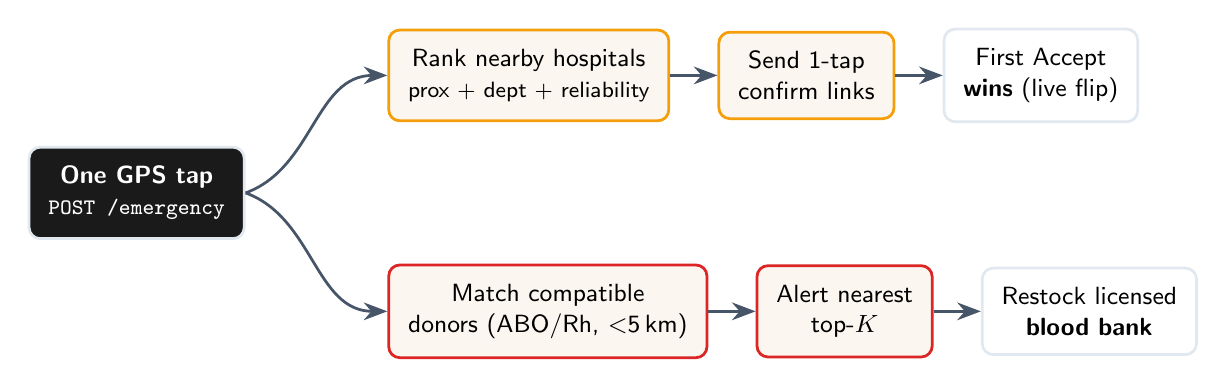
\begin{tikzpicture}[
  node distance=6mm,
  box/.style={rounded corners=4pt, draw=ghSlateLight, line width=1pt, align=center,
              font=\sffamily\small, inner sep=7pt, minimum height=1cm},
  trigger/.style={box, fill=ghInk, text=white, font=\sffamily\bfseries\small},
  hosp/.style={box, fill=ghBgSoft, draw=ghAmber},
  blood/.style={box, fill=ghBgSoft, draw=ghCrimson},
  outc/.style={box, fill=white},
  arr/.style={-{Stealth[length=3mm]}, line width=1pt, color=ghSlate}
]
\node[trigger] (trig) {One GPS tap\\\footnotesize\texttt{POST /emergency}};

\node[hosp, above right=3mm and 18mm of trig] (rank) {Rank nearby hospitals\\\footnotesize prox + dept + reliability};
\node[hosp, right=of rank] (confirm) {Send 1-tap\\confirm links};
\node[outc, right=of confirm] (flip) {First Accept\\\textbf{wins} (live flip)};

\node[blood, below right=3mm and 18mm of trig] (match) {Match compatible\\donors (ABO/Rh, $<$5\,km)};
\node[blood, right=of match] (alert) {Alert nearest\\top-$K$};
\node[outc, right=of alert] (bank) {Restock licensed\\\textbf{blood bank}};

\draw[arr] (trig.east) to[out=20,in=180] (rank.west);
\draw[arr] (rank) -- (confirm);
\draw[arr] (confirm) -- (flip);
\draw[arr] (trig.east) to[out=-20,in=180] (match.west);
\draw[arr] (match) -- (alert);
\draw[arr] (alert) -- (bank);
\end{tikzpicture}
\end{center}

\subsection{Key differentiators}
\begin{itemize}
  \item \textbf{Two lifelines, one tap, in parallel.} Routing and blood run concurrently inside one request --- not two separate apps.
  \item \textbf{Never a false bed.} The first hospital to \emph{accept} takes the patient; later acceptances are told it is already routed. The UI never shows a ``bed available'' that is not real.
  \item \textbf{Medically correct blood model.} Donors are sent to the hospital's \emph{licensed blood bank} for \emph{replacement} donation that restocks supply --- not to the patient, which is medically useless.
  \item \textbf{Works in any Indian city.} Hospitals are fetched live from OpenStreetMap (Overpass) and Google Places around the patient's actual coordinates --- the data is not seeded.
  \item \textbf{Graceful degradation.} Feature-phone SMS path, an unconfirmed-response fallback to 1-tap calling, and a demo mode that needs no external services at all.
\end{itemize}

% ===========================================================================
\section{System Architecture}

GoldenHour is a two-part system split by ownership and joined by one contract
(\code{API\_CONTRACT.md}). The frontend never touches the database; it only calls
the API. The backend is a strict three-layer design with two interchangeable data
stores behind a single factory.

\begin{center}
\begin{tikzpicture}[
  layer/.style={rounded corners=5pt, line width=1pt, align=center, font=\sffamily\small,
                inner sep=9pt, text width=13.6cm, minimum height=1.05cm},
  sub/.style={rounded corners=3pt, draw=ghSlateLight, fill=white, font=\sffamily\footnotesize,
              inner sep=5pt, align=center},
  arr/.style={-{Stealth[length=3mm]}, line width=1.2pt, color=ghSlate}
]
\node[layer, fill=ghInk, text=white] (http)
  {\textbf{HTTP layer} --- \texttt{main.py}\\[2pt]\footnotesize validate request (schema) $\rightarrow$ call \emph{one} service $\rightarrow$ return schema. No business logic.};
\node[layer, fill=ghBgSoft, draw=ghAmber, below=8mm of http] (svc)
  {\textbf{Service layer} --- \texttt{services/}\\[2pt]\footnotesize ranking \textbullet{} blood matching \textbullet{} confirmation race \textbullet{} orchestration \textbullet{} ETA \textbullet{} SMS \textbullet{} rate limiting};
\node[layer, fill=ghBgSoft, draw=ghCrimson, below=8mm of svc, minimum height=2.15cm] (data) {};
\node[anchor=north, font=\sffamily\small, text width=13cm, align=center] at ([yshift=-9pt]data.north)
  {\textbf{Data layer} --- \texttt{store.py}, one method surface behind \texttt{get\_store()}};
\node[sub, anchor=north, xshift=-3.2cm] at ([yshift=-0.85cm]data.north) (mem) {\textbf{InMemoryStore}\\seeded, haversine\\(demo / CI)};
\node[sub, anchor=north, xshift=3.2cm] at ([yshift=-0.85cm]data.north) (sup) {\textbf{SupabaseStore}\\PostgreSQL + PostGIS\\(production)};

\draw[arr] (http) -- (svc);
\draw[arr] (svc) -- (data);
\end{tikzpicture}
\end{center}

\subsection{Design rules that keep it clean}
\begin{itemize}
  \item \textbf{Routes are thin.} Each handler validates input with a Pydantic schema, calls exactly one service function, and returns a schema.
  \item \textbf{Services never touch HTTP.} They take a \code{store} plus plain values and return plain dicts --- trivially unit-testable without a client.
  \item \textbf{All data access goes through \code{store.py}.} Its method surface (\code{compatible\_donors\_nearby}, \code{create\_emergency}, \dots) is identical for both stores.
  \item \textbf{Schemas are the contract.} \code{schemas.py} mirrors \code{API\_CONTRACT.md} field-for-field; the frontend builds against the same shapes.
\end{itemize}

\subsection{Two interchangeable stores}
The radius and scoring mathematics are identical whether they run in Python
(haversine) or in PostGIS (\code{ST\_DWithin} / \code{ST\_Distance}). \code{get\_store()}
selects Supabase when \code{SUPABASE\_URL} and a key are present and reachable, and
falls back to the in-memory store otherwise --- with automatic fallback if the
client cannot be created, so boot never hard-fails. Consequences:

\begin{itemize}
  \item The demo runs end-to-end with no external services.
  \item CI needs no database.
  \item The production path (\code{sql/schema.sql} + \code{seed\_supabase.py}) is a true drop-in --- no service-code changes.
\end{itemize}

% ===========================================================================
\section{Core Algorithms}

\subsection{Hospital ranking}
For the department the emergency needs, every nearby hospital is scored and the
top $N$ (default 5) are returned, best-first:

\begin{equation*}
P(h) = 0.5 \cdot \mathrm{prox}(h) + 0.3 \cdot \mathrm{dept}(h) + 0.2 \cdot \mathrm{rel}(h)
\end{equation*}

\begin{align*}
\mathrm{prox}(h) &= \mathrm{clamp}\!\left(1 - \frac{\mathrm{eta}}{\mathrm{eta_{max}}},\, 0,\, 1\right) && \text{closer is better}\\
\mathrm{dept}(h) &= \begin{cases} 1 & \text{needed department present} \\ 0 & \text{otherwise} \end{cases} \\
\mathrm{rel}(h)  &= \text{live acceptance rate} && \text{historically reliable}
\end{align*}

\textbf{Reliability cold start.} $\mathrm{rel}(h)$ enters the score only once a
hospital has logged at least \code{REL\_ACTIVATION\_THRESHOLD} (default 20)
confirmations --- before that there is no honest reliability signal. Until then the
score degrades to proximity + department, renormalised by $0.8$ so it still spans
$[0,1]$:
\[
P(h) = \frac{0.5 \cdot \mathrm{prox}(h) + 0.3 \cdot \mathrm{dept}(h)}{0.8}.
\]
At launch (no confirmations yet) ranking is therefore pure proximity + department.
The ETA for every candidate is fetched \emph{concurrently} (see
\S\ref{sec:perf}), so latency stays flat as the candidate pool grows.

\subsection{Blood matching}
Given the requested group, the matcher selects donors who are (a) of a
\emph{compatible} group per a hardcoded ABO/Rh table, (b) available, (c) within the
search radius (default 5\,km), and (d) off their post-donation cooldown ---
\emph{sex-aware}: 90 days for men, 120 for women, per national guidelines
(\code{last\_donated IS NULL OR last\_donated < today $-$ cooldown}). The nearest
top-$K$ are alerted with directions to the hospital's \textbf{licensed blood bank}.
Rh-negative requests are flagged \code{rare\_group} so the UI can warn that supply
may be scarce.

\subsection{Confirmation race resolution}
Each ranked hospital receives a single-use one-tap link. The \textbf{first hospital
to accept} takes the patient; any later acceptance receives \code{already\_confirmed:
true} and does not override the winner. The accepted hospital flips
\code{pending $\rightarrow$ confirmed}, which the patient's screen sees via Supabase
Realtime (or polling in demo mode). If nothing confirms within
\code{UNCONFIRMED\_FALLBACK\_SECONDS} (default 180), the status response flags
\code{unconfirmed\_fallback} so the UI surfaces the nearest hospitals with a 1-tap
call --- \emph{never} a false ``bed available''.

% ===========================================================================
\section{API Design}

The API is the single source of truth both sides build against; interactive docs
are auto-generated at \code{/docs} (Swagger) and \code{/redoc}.

\begin{center}
\begin{tabularx}{\textwidth}{@{}p{5.4cm} L@{}}
\toprule
\textbf{Method \& path} & \textbf{Purpose} \\
\midrule
\code{POST /emergency} & Trigger --- rank hospitals, alert donors, send confirmation links. \\
\code{GET /emergency/\{id\}/status} & Live status --- hospital replies + donor responses (poll or Realtime). \\
\code{GET /confirm/\{token\}} & Emergency details shown on the hospital's confirmation page. \\
\code{POST /confirm/\{token\}} & Hospital taps Accept (\code{true}) / Not Available (\code{false}). \\
\code{GET /donor/respond/\{token\}} & Donor one-tap response (records intent, returns an HTML thank-you). \\
\code{POST /donor/register} & Register a replacement-blood donor (optional \code{sex} sets cooldown). \\
\code{POST /sms/inbound} & Feature-phone path --- parse an SMS, reply with nearest hospitals. \\
\code{GET /health} \textbullet{} \code{GET /ready} & Liveness (mode) \textbullet{} readiness (pings the data layer). \\
\code{GET /dev/links} \textbullet{} \code{/dev/alerts} & Demo helpers --- links sent to hospitals \textbullet{} alerts sent to donors. \\
\bottomrule
\end{tabularx}
\end{center}

\subsection{Representative request / response}
\begin{lstlisting}[language=,caption={POST /emergency --- request and response}]
// Request
{ "lat": 26.9124, "lng": 75.7873, "emergency_type": "trauma", "blood_group": "O+" }

// Response (hospitals already sorted best-first by the backend)
{
  "request_id": "abc123",
  "hospitals": [
    { "hospital_id": "h1", "name": "SMS Hospital", "lat": 26.9036, "lng": 75.8147,
      "eta_minutes": 6, "department_match": true, "distance_km": 2.3,
      "status": "pending", "phone": "+91xxxxxxxxxx" }
  ],
  "donors_alerted": 5,
  "rare_group": false
}
\end{lstlisting}

\noindent The write endpoints are rate-limited per client (fixed-window); coordinates
outside valid ranges are rejected with \code{422}; unknown tokens return \code{404}.

% ===========================================================================
\section{Frontend \& User Experience}

The PWA is a mobile-first React~19 application (Vite + Tailwind) with four screens:

\begin{itemize}
  \item \textbf{Patient Intake} --- one-tap GPS capture, emergency type and blood group.
  \item \textbf{Live Results} --- ranked hospital cards (ETA, department match, status),
  an interactive Leaflet map with the patient pin, hospital pins and route lines, a
  Golden-Hour countdown ring, and a donor-response panel.
  \item \textbf{Hospital Confirm} --- the one-tap Accept / Not Available page a hospital opens.
  \item \textbf{Donor Registration} --- name, phone, group, location, last-donated date.
\end{itemize}

\subsection{Live updates}
The results screen subscribes to Supabase Realtime for instant
\code{pending $\rightarrow$ confirmed} flips, with a 3-second polling loop as a
fallback if the socket drops. On confirmation the map auto-frames the route to the
winning hospital and a success banner slides in.

\subsection{Accessibility \& resilience}
All animation respects \code{prefers-reduced-motion} (static fallbacks for the
map ping, route lines and card transitions). The UI degrades cleanly to call links
when no hospital confirms, and the data layer's normalisation guards tolerate ETA
values arriving as either minutes or seconds.

% ===========================================================================
\section{Technology Stack}

\begin{center}
\begin{tabularx}{\textwidth}{@{}p{3.2cm} L@{}}
\toprule
\textbf{Layer} & \textbf{Technology} \\
\midrule
Frontend & React 19, Vite, Tailwind CSS, React Router, Framer Motion, Leaflet, Supabase JS client \\
Backend & Python 3.12, FastAPI, Uvicorn, Pydantic v2 \\
Database & PostgreSQL + PostGIS (via Supabase), Supabase Realtime \\
Maps / ETA & Google Maps Distance Matrix; Google Places + OpenStreetMap (Overpass) for hospital discovery \\
Messaging & Console / Telegram (demo), MSG91 / Gupshup + DLT (production) \\
Infra & Docker, Render (API), Vercel (PWA), GitHub Actions CI \\
\bottomrule
\end{tabularx}
\end{center}

% ===========================================================================
\section{Reliability, Security \& Performance}\label{sec:perf}

\begin{itemize}
  \item \textbf{Concurrent external calls.} Per-candidate ETA lookups run under
  \code{asyncio.gather}, so a busier city with more candidates does not increase
  response latency linearly --- it stays bounded by the slowest single call.
  \item \textbf{Rate limiting.} Fixed-window per-client limits guard every public
  write endpoint (\code{/emergency}, \code{/confirm}, \code{/donor/register},
  \code{/donor/respond}); excess returns \code{429}. The limiter honours
  \code{X-Forwarded-For} behind the platform proxy.
  \item \textbf{Single-use tokens.} Confirmation and donor-response links are
  URL-safe tokens, single-use; no PII beyond a phone number; secrets never reach
  the client (logging suppresses URLs that contain keys).
  \item \textbf{Health \& readiness.} \code{/health} is a cheap liveness probe that
  also accepts \code{HEAD} (for uptime monitors); \code{/ready} pings the data layer
  and returns \code{503} if the database is unreachable --- so a deploy can verify it
  is truly connected to Supabase and not silently in demo mode.
  \item \textbf{Graceful degradation.} Overpass mirrors are raced with timeouts; the
  unconfirmed-response fallback surfaces call links; the SMS path serves feature
  phones; and demo mode keeps the product fully functional with no dependencies.
\end{itemize}

% ===========================================================================
\section{Scalability}

\begin{itemize}
  \item \textbf{Stateless API.} The service holds no per-request session state, so it
  scales horizontally behind a load balancer; rate-limit state is the only in-process
  concern and is designed to back onto Redis for a multi-node deploy.
  \item \textbf{Geo at the database.} In production, donor-radius queries become real
  PostGIS \code{ST\_DWithin} lookups with spatial indexes --- the same maths as the
  demo's haversine, but executed where the data lives.
  \item \textbf{Realtime instead of polling.} Confirmations stream to the patient over
  Supabase Realtime, removing poll load at scale.
  \item \textbf{Concurrency by default.} Hospital discovery and ETA computation are
  already concurrent, so latency is governed by the slowest single upstream, not the
  candidate count.
  \item \textbf{On-demand, cached discovery.} Hospitals for a new region are fetched
  once from OSM/Places and cached per region, so the system works in \emph{any} city
  without pre-seeding all of India.
\end{itemize}

% ===========================================================================
\section{Testing \& Continuous Integration}

The suite (31 tests) runs fully offline --- no Supabase, no network --- and verifies:

\begin{itemize}
  \item the exact \code{API\_CONTRACT.md} response shapes;
  \item the ranking, blood-matching and confirmation algorithms;
  \item the end-to-end emergency $\rightarrow$ confirm $\rightarrow$ status-flip flow;
  \item the \textbf{production \code{SupabaseStore} path} against a fake Supabase client
  (\code{tests/fake\_supabase.py}), so column names, query chains and key mapping are
  validated without a live database.
\end{itemize}

\noindent CI (GitHub Actions) runs the same suite on Python 3.11 and 3.12, with lint
(\code{ruff}) and format gates enforced on every push.

% ===========================================================================
\section{Deployment}

\begin{center}
\begin{tabularx}{\textwidth}{@{}p{3.2cm} p{3.0cm} L@{}}
\toprule
\textbf{Component} & \textbf{Platform} & \textbf{Configuration} \\
\midrule
Backend API & Render (or Fly.io) & \code{render.yaml} --- Python runtime, \code{rootDir: backend}, \code{uvicorn main:app}. \\
Frontend PWA & Vercel & \code{vercel.json} --- builds \code{frontend/}, SPA rewrites. \\
Database & Supabase & Run \code{sql/schema.sql}, enable Realtime on \code{confirmation\_requests}. \\
\bottomrule
\end{tabularx}
\end{center}

\noindent Production secrets (\code{SUPABASE\_*}, \code{GOOGLE\_MAPS\_API\_KEY},
\code{MSG91\_AUTH\_KEY}, \code{VITE\_API\_BASE\_URL}) live in the respective dashboards
and are never committed. The same Docker image runs locally, in CI and in production.

% ===========================================================================
\section{Scope \& Future Work}

\textbf{Deliberately out of scope for the MVP} (integration work, not the hard problem):
real SMS gateway billing / DLT registration, hospital-staff authentication, and
ambulance dispatch integration. The hard problem --- concurrent ranking + blood
matching that works in any city, with a confirmation loop that never lies about a bed
--- is what is built and verified here.

\medskip
\noindent\textbf{Roadmap:}
\begin{itemize}
  \item Live blood-bank inventory integration (replace synthetic availability with real stock).
  \item Hospital-side dashboard and authenticated accept/decline.
  \item Production SMS with DLT-registered templates for true feature-phone reach.
  \item Redis-backed rate limiting and multi-region deployment.
\end{itemize}

% ===========================================================================
\section{Conclusion}

GoldenHour turns the single most time-critical decision in an emergency --- where to
go, and how to get blood ready --- into one tap that does both, in parallel, anywhere
in India. The engineering is honest: real data, a contract-driven architecture, a
demo that needs nothing, and a production path that is a configuration switch rather
than a rewrite. It is not a directory and not a donor list; it is a dispatch system
for the hour that decides.

% ---------- Appendix -------------------------------------------------------
\appendix
\section{Appendix --- Configuration Reference}

\begin{center}
\begin{tabularx}{\textwidth}{@{}p{5.8cm} p{2.2cm} L@{}}
\toprule
\textbf{Variable} & \textbf{Default} & \textbf{Effect} \\
\midrule
\code{SUPABASE\_URL} + key & --- & Set $\rightarrow$ use the real database (else demo). \\
\code{GOOGLE\_MAPS\_API\_KEY} & --- & Set $\rightarrow$ real drive-time ETAs and Places discovery. \\
\code{FRONTEND\_URL} & localhost:5173 & Base for \code{/confirm/<token>} links. \\
\code{DONOR\_RADIUS\_METERS} & 5000 & Donor search radius. \\
\code{DONOR\_COOLDOWN\_DAYS} & 90 & Post-donation cooldown (men / default). \\
\code{DONOR\_COOLDOWN\_DAYS\_FEMALE} & 120 & Post-donation cooldown (women). \\
\code{DONOR\_ALERT\_K} & 10 & Nearest matched donors actually alerted. \\
\code{REL\_ACTIVATION\_THRESHOLD} & 20 & Confirmations before \code{rel(h)} counts. \\
\code{UNCONFIRMED\_FALLBACK\_SECONDS} & 180 & No-confirmation window before the 1-tap-call fallback. \\
\code{RANKING\_TOP\_N} & 5 & Hospitals returned per emergency. \\
\bottomrule
\end{tabularx}
\end{center}

\vfill
\begin{center}
{\sffamily\color{ghSlate}\small GoldenHour --- Bharat Academix CodeQuest 2026 --- MVP Technical Documentation}
\end{center}

\end{document}
